\chapter{Background}
\chlabel{Background}


\section{The GROOVE project}

\GROOVE is an acronym of {\bf GR}aphs for {\bf O}bject {\bf O}riented {\bf VE}rification. In this project we work towards a method in which graphs are used for describing the structure of states of object-oriented programs. Such states mainly consist of objects that have been created during execution and their inter-relationships.

If each of the state of such a program is modelled by a single graph, the quesion is still how to relate (or order) all these graphs in a meaningful way. The obvious relation to chose is their temporal appearance. In other words, graphs representing subsequent states of a program should be related.

These relations between states are specified as applications of {\em graph transformation rules}. Intuitively, a graph transformation rule specifies how to make (local) changes to a certain graph. More formally, a graph transformation rule consists of a left hand side graph (\lhs) and a right hand side graph (\rhs) together with a graph morphism mapping elements of \lhs to elements of \rhs and a set of {\nac}s, being supergraphs of \lhs. It is not our intention to give an introduction to this field in this document, but rather refer to \cite{Heckel2006} which contains sufficient pointers for further reading.


\section{The GROOVE Approach}

Within the \GROOVE Tool Set the theory of graph transformation is applied on what are often called {\em simple graphs}. Simple graphs, as graphs in general, consists of a set of {\em nodes} and a set of {\em edges}. Edges, however, do not have an identity, but are identified by their {\em source node}, {\em target node}, and {\em label} instead. Therefore, edges with the same source node, target node, and label necessarily need to be equal, or stated differently, {\em parallel edges} are not allowed.

In \cite{GG-Handbook-I} the two main graph transformation approaches, namely the Single Pushout (\spo) and the Double Pushout (\dpo) approach, are explained and compared in detail. In \GROOVE we apply the \spo approach, mainly because the \dpo approach is not defined on simple graphs with partial graph morphisms. Shortly, the \spo approach unconditionally applies the graph transformation rules. If then, rule applications result in ill-formed graphs, i.e. graphs containing {\em dangling edges} for which either their source node or target node is not defined, those graphs are made well-formed again by removing the ill-formed part, i.e. by removing those dangling edges.

\section{Visualizing Transformation Rules}

Traditional graph transformation approaches specify a transformation rule by showing each component, i.e. its \lhs, \rhs, and all {\nac}s, separately. \fref{traditional-rule} is an example of such a traditional way of specifying a transformation rule. Graph morphisms are typically defined by means of the placing of the graph elements (i.e. nodes and edges).

\begin{figure}[htp]
  \centering
  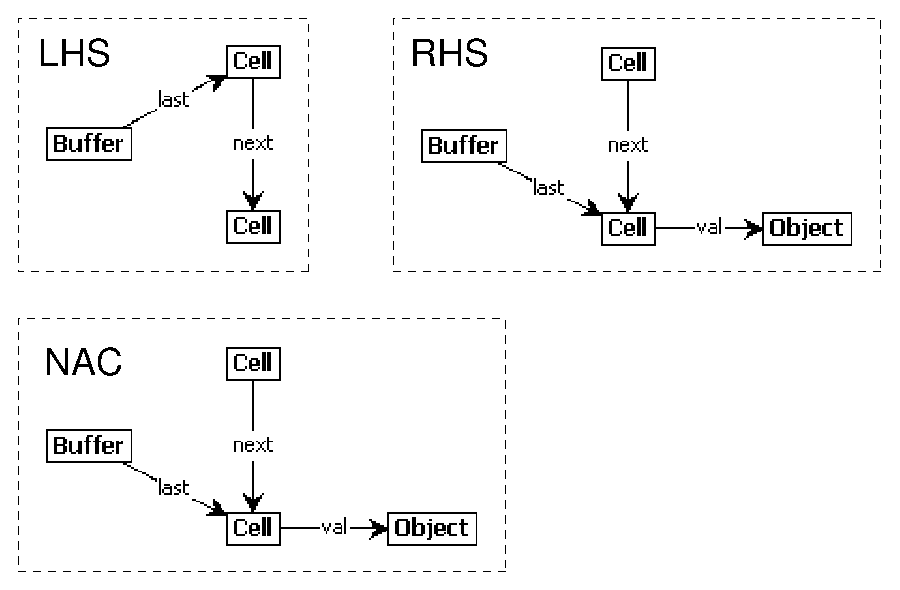
\includegraphics[scale=.75]{\figdir/traditional-rule}
  \caption{Traditional representation of a transformation rule.}
  \flabel{traditional-rule}
\end{figure}

In the GROOVE Tool Set we use a single graph representation of transformation rules. In this we depict the different roles of the graph elements by using different shapes and colours. We distinguish between four roles:

\begin{itemize}
  \item{{\em reader}: these are the nodes and edges that are only read by the rule, i.e. they are both in \lhs and \rhs. Reader nodes and edges are depicted as solid, black rectangles and arrows;}
  \item{{\em erasor}: these are the nodes and edges that are removed by the rule, i.e. they are only in \lhs. Erasor nodes and edges are represented by blue, dashed rectangles and arrows;}
  \item{{\em creator}: these are the nodes and edges that are created by the rule, i.e. they are only in \rhs. Creator nodes and edges are represented by solid, fat, green rectangles and arrows;}
  \item{{\em embargoe}: these are the nodes and edges that are forbidden for the rule to be applicable, i.e. they must not be present in the graph on which we want the rule to be applicable. Embargoe nodes and edges are represented by solid, fat, red rectangles and arrows.}
\end{itemize}

In \fref{groove-rule}, the single graph representation of the rule from \fref{traditional-rule} is shown.

\begin{figure}[htp]
  \centering
  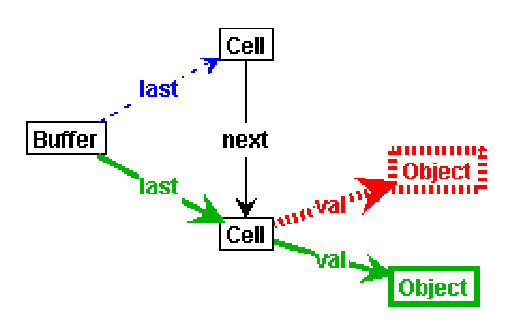
\includegraphics[scale=0.75]{\figdir/groove-rule}
  \caption{The GROOVE's single graph representation of \fref{traditional-rule}.}
  \flabel{groove-rule}
\end{figure}

